\documentclass[../main]{subfiles}

\questiontrue
\solutiontrue

\begin{document}
    \ifquestion
    
	\section{Binary Systems}

In this problem, we aim to find the shape of the orbits of binary systems. After all, Kepler's basic laws referred only to a system where one body was considerably more massive and therefore remained practically stationary, so why should the orbits of binaries be ellipses? Obviously, we already know this fact, but understanding this reason will be very useful in the future.

\begin{doublespace}

\begin{large}
\textbf{Part A: Orbital Parameters}
\end{large}

\end{doublespace}

Consider two bodies in the plane, as shown in the figure below:

	\begin{figure}[htpb]
	    \centering
	    

\tikzset{every picture/.style={line width=0.75pt}} %set default line width to 0.75pt        

\begin{tikzpicture}[x=0.75pt,y=0.75pt,yscale=-1,xscale=1]
%uncomment if require: \path (0,408); %set diagram left start at 0, and has height of 408

%Shape: Circle [id:dp8037274103794245] 
\draw  [fill={rgb, 255:red, 6; green, 18; blue, 207 }  ,fill opacity=1 ] (174,288.83) .. controls (174,281.75) and (179.75,276) .. (186.83,276) .. controls (193.92,276) and (199.67,281.75) .. (199.67,288.83) .. controls (199.67,295.92) and (193.92,301.67) .. (186.83,301.67) .. controls (179.75,301.67) and (174,295.92) .. (174,288.83) -- cycle ;
%Shape: Circle [id:dp37942559470955994] 
\draw  [fill={rgb, 255:red, 208; green, 2; blue, 27 }  ,fill opacity=1 ] (403.33,126.5) .. controls (403.33,124.01) and (405.35,122) .. (407.83,122) .. controls (410.32,122) and (412.33,124.01) .. (412.33,126.5) .. controls (412.33,128.99) and (410.32,131) .. (407.83,131) .. controls (405.35,131) and (403.33,128.99) .. (403.33,126.5) -- cycle ;
%Straight Lines [id:da5035300847814483] 
\draw [color={rgb, 255:red, 4; green, 17; blue, 140 }  ,draw opacity=1 ]   (264.27,231.95) -- (198.62,279.5) ;
\draw [shift={(197,280.67)}, rotate = 324.08] [color={rgb, 255:red, 4; green, 17; blue, 140 }  ,draw opacity=1 ][line width=0.75]    (10.93,-3.29) .. controls (6.95,-1.4) and (3.31,-0.3) .. (0,0) .. controls (3.31,0.3) and (6.95,1.4) .. (10.93,3.29)   ;
%Straight Lines [id:da5088332383250584] 
\draw [color={rgb, 255:red, 208; green, 2; blue, 27 }  ,draw opacity=1 ]   (264.27,231.95) -- (401.96,130.43) ;
\draw [shift={(403.57,129.25)}, rotate = 143.6] [color={rgb, 255:red, 208; green, 2; blue, 27 }  ,draw opacity=1 ][line width=0.75]    (10.93,-3.29) .. controls (6.95,-1.4) and (3.31,-0.3) .. (0,0) .. controls (3.31,0.3) and (6.95,1.4) .. (10.93,3.29)   ;
%Shape: Circle [id:dp30585639099704176] 
\draw  [fill={rgb, 255:red, 0; green, 0; blue, 0 }  ,fill opacity=1 ] (263.06,231.95) .. controls (263.06,231.28) and (263.6,230.73) .. (264.27,230.73) .. controls (264.94,230.73) and (265.49,231.28) .. (265.49,231.95) .. controls (265.49,232.62) and (264.94,233.16) .. (264.27,233.16) .. controls (263.6,233.16) and (263.06,232.62) .. (263.06,231.95) -- cycle ;
%Straight Lines [id:da06222451152050712] 
\draw [color={rgb, 255:red, 4; green, 17; blue, 140 }  ,draw opacity=1 ]   (198,293.42) -- (254.14,315.68) ;
\draw [shift={(256,316.42)}, rotate = 201.63] [color={rgb, 255:red, 4; green, 17; blue, 140 }  ,draw opacity=1 ][line width=0.75]    (10.93,-3.29) .. controls (6.95,-1.4) and (3.31,-0.3) .. (0,0) .. controls (3.31,0.3) and (6.95,1.4) .. (10.93,3.29)   ;
%Straight Lines [id:da34723906504840363] 
\draw [color={rgb, 255:red, 208; green, 2; blue, 27 }  ,draw opacity=1 ]   (275.85,70.19) -- (404.5,123.77) ;
\draw [shift={(274,69.42)}, rotate = 22.61] [color={rgb, 255:red, 208; green, 2; blue, 27 }  ,draw opacity=1 ][line width=0.75]    (10.93,-3.29) .. controls (6.95,-1.4) and (3.31,-0.3) .. (0,0) .. controls (3.31,0.3) and (6.95,1.4) .. (10.93,3.29)   ;

% Text Node
\draw (144.5,273.07) node [anchor=north west][inner sep=0.75pt]  [font=\large,color={rgb, 255:red, 23; green, 7; blue, 162 }  ,opacity=1 ]  {$m_{2}$};
% Text Node
\draw (217.5,221.07) node [anchor=north west][inner sep=0.75pt]  [font=\large,color={rgb, 255:red, 23; green, 7; blue, 162 }  ,opacity=1 ]  {$\vec{r}_{2}$};
% Text Node
\draw (245,286.07) node [anchor=north west][inner sep=0.75pt]  [font=\large,color={rgb, 255:red, 23; green, 7; blue, 162 }  ,opacity=1 ]  {$\vec{v}_{2}$};
% Text Node
\draw (416,103.57) node [anchor=north west][inner sep=0.75pt]  [font=\large,color={rgb, 255:red, 208; green, 2; blue, 27 }  ,opacity=1 ]  {$m_{1}$};
% Text Node
\draw (341.5,176.17) node [anchor=north west][inner sep=0.75pt]  [font=\large,color={rgb, 255:red, 208; green, 2; blue, 27 }  ,opacity=1 ]  {$\vec{r}_{1}$};
% Text Node
\draw (334.5,66.57) node [anchor=north west][inner sep=0.75pt]  [font=\large,color={rgb, 255:red, 208; green, 2; blue, 27 }  ,opacity=1 ]  {$\vec{v}_{1}$};


\end{tikzpicture}
	    \caption{Binary System}
	    \label{fig:bina}
	\end{figure}


\ut{A.1} Find an expression for the gravitational force experienced between the bodies.

\ut{A.2} Remember that the center of mass in an isolated system moves with uniform velocity (use $v=0$ without loss of generality). In this case, use the following trick: Suppose there were a body of mass $m_x$ at the center of mass and only this body acted on $m_i$ ($i \in \lbrace 1,2 \rbrace$), what should the value of $m_x$ be so that the orbit of $m_i$ is the same as in the previous case? Denote $m_j$ as the other component of the binary system.

\ut{A.3} Prove that the orbit is a conic section and find the values of $a_1$ and $e_1$ in terms of the velocity $v_{p,1}$ (velocity of body 1 at periapsis) and $L$, the minimum separation between the components. Then, show that $m_1a_1=m_2a_2$ and that $e_1=e_2=e$.

\begin{doublespace}

\begin{large}
\textbf{Part B: Relative Orbits}
\end{large}

\end{doublespace}

\ut{B.1} Write the total mechanical energy equation of the system in terms of the relative velocity $V$ of one star as seen from the other, $M$, the sum of the component masses, $\mu=\frac{m_1m_2}{m_1+m_2}$, the reduced mass of the system, and $L$, the distance between the components.

\ut{B.2} Reinterpret the result from the concept of relative orbit. What does each parameter represent?

\begin{doublespace}

\begin{large}
\textbf{Part C: Lagrangian Points}
\end{large}

\end{doublespace}

Lagrangian points are points where, if a small test mass $m \ll m_1, m_2$ were placed, it would orbit with the same angular velocity as the system, that is, it would have the same orbital period and therefore would "follow" the revolutions of the binary. Get ready for the calculations!
	
	\begin{figure}[htpb]
	    \centering
	    

\tikzset{every picture/.style={line width=0.75pt}} %set default line width to 0.75pt        

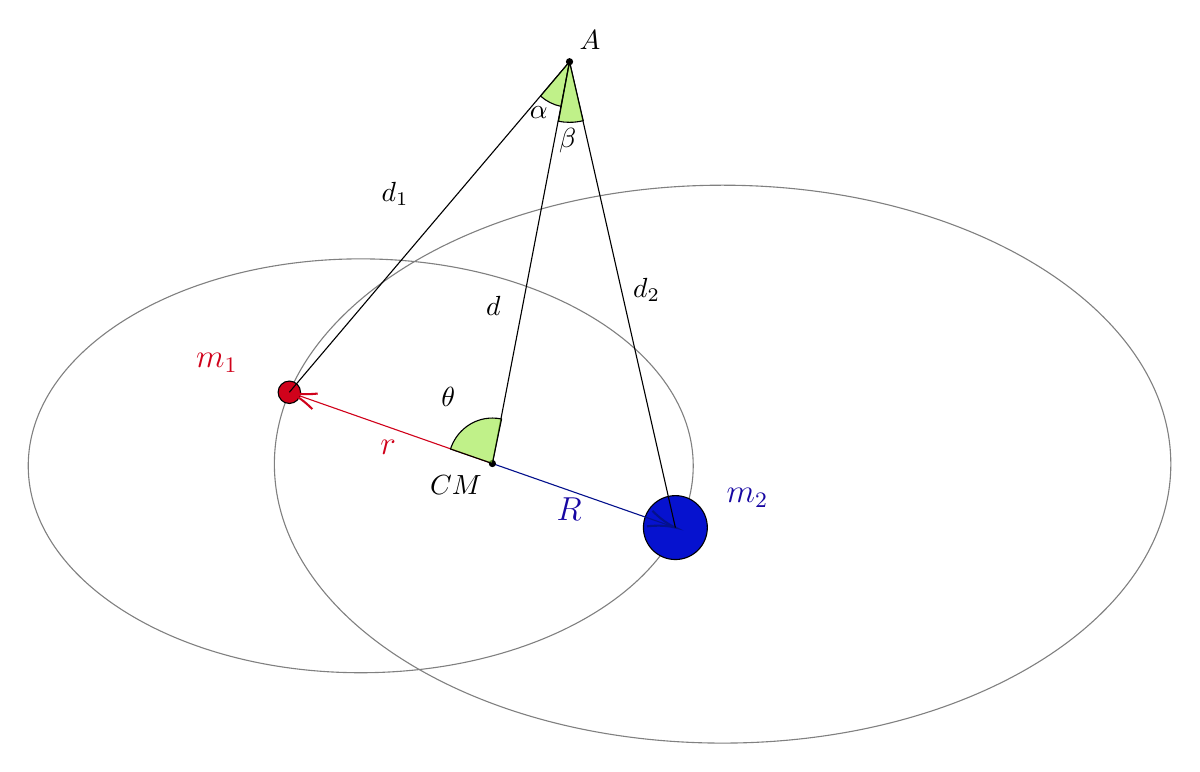
\begin{tikzpicture}[x=0.75pt,y=0.75pt,yscale=-1.2,xscale=1.2]
%uncomment if require: \path (0,408); %set diagram left start at 0, and has height of 408

%Shape: Ellipse [id:dp09117954938881878] 
\draw  [color={rgb, 255:red, 128; green, 128; blue, 128 }  ,draw opacity=1 ][fill={rgb, 255:red, 155; green, 155; blue, 155 }  ,fill opacity=0 ] (99.67,187.09) .. controls (99.67,141.2) and (159.44,104) .. (233.17,104) .. controls (306.9,104) and (366.67,141.2) .. (366.67,187.09) .. controls (366.67,232.97) and (306.9,270.17) .. (233.17,270.17) .. controls (159.44,270.17) and (99.67,232.97) .. (99.67,187.09) -- cycle ;
%Shape: Ellipse [id:dp34920972297135533] 
\draw  [color={rgb, 255:red, 128; green, 128; blue, 128 }  ,draw opacity=1 ][fill={rgb, 255:red, 155; green, 155; blue, 155 }  ,fill opacity=0 ] (198.5,186.42) .. controls (198.5,124.56) and (279.07,74.42) .. (378.46,74.42) .. controls (477.85,74.42) and (558.42,124.56) .. (558.42,186.42) .. controls (558.42,248.28) and (477.85,298.42) .. (378.46,298.42) .. controls (279.07,298.42) and (198.5,248.28) .. (198.5,186.42) -- cycle ;
%Shape: Circle [id:dp0009033171380325999] 
\draw  [fill={rgb, 255:red, 6; green, 18; blue, 207 }  ,fill opacity=1 ] (346.67,211.89) .. controls (346.67,204.8) and (352.41,199.06) .. (359.5,199.06) .. controls (366.59,199.06) and (372.33,204.8) .. (372.33,211.89) .. controls (372.33,218.98) and (366.59,224.72) .. (359.5,224.72) .. controls (352.41,224.72) and (346.67,218.98) .. (346.67,211.89) -- cycle ;
%Shape: Circle [id:dp3324641980057337] 
\draw  [fill={rgb, 255:red, 208; green, 2; blue, 27 }  ,fill opacity=1 ] (200,157.56) .. controls (200,155.07) and (202.01,153.06) .. (204.5,153.06) .. controls (206.99,153.06) and (209,155.07) .. (209,157.56) .. controls (209,160.04) and (206.99,162.06) .. (204.5,162.06) .. controls (202.01,162.06) and (200,160.04) .. (200,157.56) -- cycle ;
%Straight Lines [id:da772726484090762] 
\draw [color={rgb, 255:red, 4; green, 17; blue, 140 }  ,draw opacity=1 ]   (286.02,186.17) -- (357.61,211.23) ;
\draw [shift={(359.5,211.89)}, rotate = 199.29] [color={rgb, 255:red, 4; green, 17; blue, 140 }  ,draw opacity=1 ][line width=0.75]    (10.93,-3.29) .. controls (6.95,-1.4) and (3.31,-0.3) .. (0,0) .. controls (3.31,0.3) and (6.95,1.4) .. (10.93,3.29)   ;
%Straight Lines [id:da3526235569897358] 
\draw [color={rgb, 255:red, 208; green, 2; blue, 27 }  ,draw opacity=1 ]   (286.02,186.17) -- (206.39,158.22) ;
\draw [shift={(204.5,157.56)}, rotate = 19.34] [color={rgb, 255:red, 208; green, 2; blue, 27 }  ,draw opacity=1 ][line width=0.75]    (10.93,-3.29) .. controls (6.95,-1.4) and (3.31,-0.3) .. (0,0) .. controls (3.31,0.3) and (6.95,1.4) .. (10.93,3.29)   ;
%Shape: Circle [id:dp5215426804924401] 
\draw  [fill={rgb, 255:red, 0; green, 0; blue, 0 }  ,fill opacity=1 ] (284.81,186.17) .. controls (284.81,185.5) and (285.35,184.96) .. (286.02,184.96) .. controls (286.69,184.96) and (287.24,185.5) .. (287.24,186.17) .. controls (287.24,186.84) and (286.69,187.38) .. (286.02,187.38) .. controls (285.35,187.38) and (284.81,186.84) .. (284.81,186.17) -- cycle ;
%Straight Lines [id:da8982454011809149] 
\draw    (317,24.85) -- (204.5,157.56) ;
%Straight Lines [id:da7953076021679728] 
\draw    (317,24.85) -- (359.5,211.89) ;
%Straight Lines [id:da20080138743090137] 
\draw    (317,24.85) -- (286.02,186.17) ;
%Shape: Circle [id:dp688841400360662] 
\draw  [fill={rgb, 255:red, 0; green, 0; blue, 0 }  ,fill opacity=1 ] (315.79,24.85) .. controls (315.79,24.18) and (316.33,23.64) .. (317,23.64) .. controls (317.67,23.64) and (318.21,24.18) .. (318.21,24.85) .. controls (318.21,25.52) and (317.67,26.06) .. (317,26.06) .. controls (316.33,26.06) and (315.79,25.52) .. (315.79,24.85) -- cycle ;
%Shape: Pie [id:dp795785269312111] 
\draw  [fill={rgb, 255:red, 145; green, 230; blue, 48 }  ,fill opacity=0.57 ] (269.2,180.35) .. controls (271.56,173.12) and (278.2,167.91) .. (286.02,167.91) .. controls (287.29,167.91) and (288.52,168.05) .. (289.71,168.3) -- (286.02,186.17) -- cycle ;
%Shape: Pie [id:dp15400864576342577] 
\draw  [fill={rgb, 255:red, 145; green, 230; blue, 48 }  ,fill opacity=0.57 ] (313.55,42.77) .. controls (310.46,42.14) and (307.65,40.68) .. (305.36,38.63) -- (317,24.85) -- cycle ;
%Shape: Pie [id:dp12314152432146308] 
\draw  [fill={rgb, 255:red, 145; green, 230; blue, 48 }  ,fill opacity=0.57 ] (322.5,48.52) .. controls (320.74,48.96) and (318.89,49.18) .. (317,49.18) .. controls (315.49,49.18) and (314.01,49.04) .. (312.57,48.76) -- (317,24.85) -- cycle ;

% Text Node
\draw (379,194.96) node [anchor=north west][inner sep=0.75pt]  [font=\large,color={rgb, 255:red, 23; green, 7; blue, 162 }  ,opacity=1 ]  {$m_{2}$};
% Text Node
\draw (310.75,198.71) node [anchor=north west][inner sep=0.75pt]  [font=\large,color={rgb, 255:red, 23; green, 7; blue, 162 }  ,opacity=1 ]  {$R$};
% Text Node
\draw (166,140.96) node [anchor=north west][inner sep=0.75pt]  [font=\large,color={rgb, 255:red, 208; green, 2; blue, 27 }  ,opacity=1 ]  {$m_{1}$};
% Text Node
\draw (240,175.56) node [anchor=north west][inner sep=0.75pt]  [font=\large,color={rgb, 255:red, 208; green, 2; blue, 27 }  ,opacity=1 ]  {$r$};
% Text Node
\draw (260,190.07) node [anchor=north west][inner sep=0.75pt]    {$CM$};
% Text Node
\draw (320,11.4) node [anchor=north west][inner sep=0.75pt]    {$A$};
% Text Node
\draw (282.5,118.07) node [anchor=north west][inner sep=0.75pt]    {$d$};
% Text Node
\draw (240.5,72.07) node [anchor=north west][inner sep=0.75pt]    {$d_{1}$};
% Text Node
\draw (341.5,110.57) node [anchor=north west][inner sep=0.75pt]    {$d_{2}$};
% Text Node
\draw (264.5,154.57) node [anchor=north west][inner sep=0.75pt]  [color={rgb, 255:red, 0; green, 0; blue, 0 }  ,opacity=1 ]  {$\theta $};
% Text Node
\draw (300,41.87) node [anchor=north west][inner sep=0.75pt]    {$\alpha $};
% Text Node
\draw (311.75,50.37) node [anchor=north west][inner sep=0.75pt]    {$\beta $};


\end{tikzpicture}
	
\caption{Components of the binary system ($m_1$ and $m_2$) and the Lagrangian point $A$}
\label{fig:lagrange}
\end{figure}

Consider the binary system such that, at a given moment, body $m_1$ is located at a distance $r$ from the center of mass (CM) and $m_2$ at a distance $R$. Consider point A in the figure as a small test mass such that it has an orbit around the center of mass with the same period as the binary, equal to $T$. We wish to find the parameters that allow the existence of this orbit.

Thus, we have 2 cases: the case where $\sin{(\theta)}=0$ ($\theta \in \lbrace 0,180^\circ \rbrace$), i.e., all three are aligned, and the case where $\sin{(\theta)} \neq 0$, where they are not aligned. In the following problems, the non-alignment cases of the Lagrangian point will be discussed. The other points are left as an exercise to the reader (checkmate!).

There are two points that satisfy this condition and they are symmetric with respect to the line connecting the components, so we only need to find one of them.

\ut{C.1} Given the gravitational forces of $m_1$ and $m_2$ on $A$, find a relation for the components parallel to $d$ and perpendicular to $d$. Again, use the trick that the orbit of $A$ will be dictated by a body of mass $m_x$, which will be determined during the calculations.

\ut{C.2} Prove that $d_1=d_2=D$ and that $d=kD$. Show the value of $k$ in terms of $m_x$, $m_1$, and $m_2$. Hint: Recall the law of sines and the law of cosines.

\ut{C.3} Relate the values of $a_x$ and $m_x$ with $a_1$, $a_2$, $m_1$, and $m_2$ using Kepler’s third law, where $a_1$ and $a_2$ are the semimajor axes of the orbits of $m_1$ and $m_2$. Finally, show that $a_x=k(a_1+a_2)$.

\ut{C.4} Find the eccentricity of $A$’s orbit from the calculation of the periapsis and apoapsis positions of $A$’s orbit. Hint: Recall the relation of $d$ with $L$.

\ut{C.5} Finally, relate the different equations for calculating $a_x$ and determine the value of $k$. Also show the values of $\cos{(\theta)}$, $m_x$, and $d$. Notice that since the value of angle $\theta$ is constant, the object maintains a constant angular position in the binary reference frame, which is precisely the condition for a Lagrangian point!

\ut{C.6} Show that $D=L$ and, therefore, the triangle $\Delta A,m_1,m_2$ is an equilateral triangle!

\textbf{Bonus:} it is possible to extend the previous result to any conic!

\clearpage

\fi

\ifsolution

\section{Binary Systems}

\begin{doublespace}

\begin{large}
\textbf{Part A: Orbital Parameters}
\end{large}

\end{doublespace}

\ut{A.1} Just use the universal law of gravitation:

$$|\vec{F}|=\frac{Gm_1m_2}{(r_1+r_2)^2}$$

\ut{A.2} Consider that the point between the masses is the center of mass. Recall the definition of center of mass:

\begin{equation}
\vec{x}_{CM}=\frac{\sum_i m_i \vec{x}_i}{M}
\label{d}
\end{equation}

If we define the center of mass as the origin of the Cartesian plane, in this example we notice that:

$$\vec{x}_{CM}=0=\frac{m_1\vec{r}_1+m_2\vec{r}_2}{m_1+m_2}$$

Thus we find:

\begin{equation}
m_1|\vec{r}_1|=m_2|\vec{r}_2|
\label{e}
\end{equation}

If we take the time derivative of both sides (remember that the time derivative of position is velocity):

$$\frac{d}{dt} m_1 \vec{r}_1 = \frac{d}{dt} m_2 \vec{r}_2$$

$$\frac{dm_1}{dt}\vec{r}_1 + m_1\vec{v}_1 = \frac{dm_2}{dt}\vec{r}_2 + m_2\vec{v}_2$$

Since the masses of the components do not vary, we can set the time derivatives of the masses to 0:

\begin{equation}
m_1 \vec{v}_1 = m_2 \vec{v}_2
\label{f}
\end{equation}

Equations \lab{f} and \lab{e} reveal important facts: the ratios of velocities and positions relative to the center of mass depend on the component masses, and equally important, the velocities are parallel and the position vectors are collinear (you can see this since the velocity and position vectors are linearly dependent, i.e., one is a multiple of the other).

Now considering the force acting on body $m_i$:

$$\vec{F}_{ji}=-\frac{Gm_im_j}{(r_i+r_j)^2}\hat{r_i}$$

Notice that, by equation \lab{e}, we can rewrite $r_j$ as $\frac{m_i r_i}{m_j}$, then we have:

$$\vec{F}_{ji}=-\frac{G m_i m_j}{(r_i + \frac{m_i r_i}{m_j})^2} \hat{r_i} = -\frac{G m_i m_j^3}{(m_i+m_j)^2 r_i^2} \hat{r_i}$$

In the case of a fixed central mass $m_x$:

$$\vec{F}_{ji}=-\frac{G m_i m_x}{r_i^2} \hat{r_i}$$

Thus, we see that:

$$m_x = \frac{m_j^3}{(m_i+m_j)^2}$$

\ut{A.3} In this analysis, the orbit of body $i$ is "identical" to this fictitious orbit where the central body is fixed at the center of mass. This result is great because it ensures that each component of the binary orbits in an ellipse, allowing us to apply the well-known Kepler laws.

Using this technique, we can find some orbital parameters of each component. First, we can find the semimajor axis of the orbit from the total mechanical energy equation:

$$\frac{1}{2} m_1 v_{p,1}^2 - \frac{G m_1 m_2^3}{(m_1+m_2)^2 r_{p,1}} = -\frac{G m_1 m_2^3}{(m_1+m_2)^2 a_1}$$

Since $m_1 r_{p,1} = m_2 r_{p,2}$ and $r_{p,1}+r_{p,2}=L$, we find:

$$r_{p,1} = \frac{m_2 L}{m_1+m_2}$$

Thus we find:

$$a_1 = \frac{G m_2^3 L}{4 G m_2^2 (m_1+m_2) - 2 v_{p,1}^2 L (m_1+m_2)^2}$$

By the vis-viva equation, we have:

$$v_p = \sqrt{G \frac{m_2^3}{(m_1+m_2)^2} \left( \frac{2}{a_1(1-e_1)} - \frac{1}{a_1} \right)}$$

$$v_{p,1} r_{p,1} = \sqrt{G \frac{m_2^3}{(m_1+m_2)^2} a_1 (1-e_1^2)}$$

Thus:

$$e_1^2 = 1 - 2 \frac{v_{p,1}^2 L (m_1+m_2)}{G m_2^2} + \frac{v_{p,1}^4 L^2 (m_1+m_2)^2}{G^2 m_2^4}$$

Simplifying:

$$e_1 = \frac{v_{p,1}^2 L (m_1+m_2)}{G m_2^2} - 1$$

Notice that $v_{p,1}^2 = \frac{(m_1 v_{p,1})^2}{m_1^2}$, so:

$$e_1 = \frac{(m_1 v_{p,1})^2 L (m_1+m_2)}{G m_2^2 m_1^2} - 1$$

Doing the same for body $m_2$ (swap indices):

$$e_1 = \frac{(m_2 v_{p,2})^2 L (m_2+m_1)}{G m_1^2 m_2^2} - 1$$

Since $m_1 v_{p,1} = m_2 v_{p,2}$, all expressions are identical:

$$e_1 = e_2$$

At periapsis:

$$m_1 a_1 (1-e_1) = m_2 a_2 (1-e_2)$$

And since $e_1=e_2$, we have $m_1 a_1 = m_2 a_2$.

\begin{doublespace}

\begin{large}
\textbf{Part B: Relative Orbits}
\end{large}

\end{doublespace}

\ut{B.1} In this situation, the relative position of $m_2$ with respect to $m_1$ is $\vec{L} = \vec{r}_2 - \vec{r}_1$ and the relative velocity is (neglecting relativistic effects) $\vec{V} = \vec{v}_2 - \vec{v}_1$, but what really matters is the magnitude of these parameters ($L = r_1 + r_2$ and $V = v_1 + v_2$).

Thus, we write the energy equation of the system in terms of these relative parameters:

$$E_m = \frac{1}{2} m_2 v_2^2 + \frac{1}{2} m_1 v_1^2 - \frac{G m_1 m_2}{r_1+r_2}$$

Note that $V = v_2 + \frac{m_2 v_2}{m_1}$, therefore $v_2 = \frac{m_1 V}{m_1+m_2}$, analogously $v_1 = \frac{m_2 V}{m_1+m_2}$. Let $M = m_1+m_2$:

$$E_m = \frac{1}{2} \frac{m_2 m_1^2}{M^2} V^2 + \frac{1}{2} \frac{m_1 m_2^2}{M^2} V^2 - \frac{G m_1 m_2}{R}$$

Simplifying:

$$E_m = \frac{1}{2} \frac{m_1 m_2}{M} V^2 - \frac{G m_1 m_2}{R}$$

Rewrite: $m_1 m_2 = \frac{m_1 m_2 M}{M}$:

$$E_m = \frac{1}{2} \mu V^2 - \frac{G \mu M}{R}$$

with $\mu = \frac{m_1 m_2}{m_1+m_2}$, the reduced mass of the system.

\ut{B.2} Notice that this relation is identical to that of a body of mass $\mu$ orbiting a fixed central mass $M$, with relative parameters ($L$ and $V$). Therefore, the relative orbit of one star with respect to the other can be modeled as this auxiliary orbit.

\begin{doublespace}

\begin{large}
\textbf{Part C: Lagrangian Points}
\end{large}

\end{doublespace}

\ut{C.1} First, note that the resultant gravitational force between $A$, $m_1$ and $A$, $m_2$ must point toward the center of mass (under our conditions), so the forces in directions perpendicular to the line connecting $A$ and CM must cancel:

$$F_{A,m_1} \sin{(\alpha)} = F_{A,m_2} \sin{(\beta)}$$

$$\frac{G m_1 m_A}{d_1^2} \sin{(\alpha)} = \frac{G m_2 m_A}{d_2^2} \sin{(\beta)}$$

\begin{equation}
\frac{m_1}{d_1^2} \sin{(\alpha)} = \frac{m_2}{d_2^2} \sin{(\beta)}
\label{g}
\end{equation}

On the other hand, the sum of the forces in the direction of the center of mass must result in a gravitational force that puts body $A$ in the desired orbit of period $T$:

$$F_{A,m_1} \cos{(\alpha)} + F_{A,m_2} \cos{(\beta)} = F_{A,CM}$$

$$\frac{G m_1 m_A}{D^2} \cos{(\alpha)} + \frac{G m_2 m_A}{D^2} \cos{(\beta)} = \frac{G m_x m_A}{d^2}$$

Notice that $m_x$ is used to represent the effective mass that would attract $m_A$. Thus:

	\begin{equation}
		\frac{m_1}{D^2}\cos{(\alpha)}+\frac{m_2}{D^2}\cos{(\beta)}=\frac{m_x}{d^2}
		\label{h}
	\end{equation}
	
	\begin{figure}[htpb]
	    \centering
	    \tikzset{every picture/.style={line width=0.75pt}} %set default line width to 0.75pt        

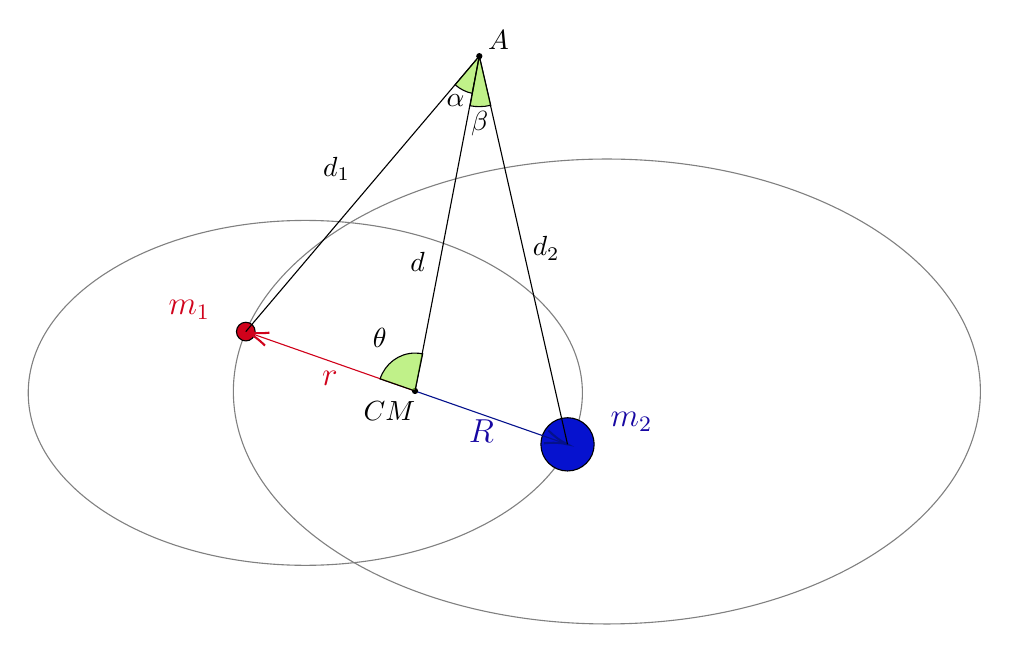
\begin{tikzpicture}[x=0.75pt,y=0.75pt,yscale=-1,xscale=1]
%uncomment if require: \path (0,408); %set diagram left start at 0, and has height of 408

%Shape: Ellipse [id:dp09117954938881878] 
\draw  [color={rgb, 255:red, 128; green, 128; blue, 128 }  ,draw opacity=1 ][fill={rgb, 255:red, 155; green, 155; blue, 155 }  ,fill opacity=0 ] (99.67,187.09) .. controls (99.67,141.2) and (159.44,104) .. (233.17,104) .. controls (306.9,104) and (366.67,141.2) .. (366.67,187.09) .. controls (366.67,232.97) and (306.9,270.17) .. (233.17,270.17) .. controls (159.44,270.17) and (99.67,232.97) .. (99.67,187.09) -- cycle ;
%Shape: Ellipse [id:dp34920972297135533] 
\draw  [color={rgb, 255:red, 128; green, 128; blue, 128 }  ,draw opacity=1 ][fill={rgb, 255:red, 155; green, 155; blue, 155 }  ,fill opacity=0 ] (198.5,186.42) .. controls (198.5,124.56) and (279.07,74.42) .. (378.46,74.42) .. controls (477.85,74.42) and (558.42,124.56) .. (558.42,186.42) .. controls (558.42,248.28) and (477.85,298.42) .. (378.46,298.42) .. controls (279.07,298.42) and (198.5,248.28) .. (198.5,186.42) -- cycle ;
%Shape: Circle [id:dp0009033171380325999] 
\draw  [fill={rgb, 255:red, 6; green, 18; blue, 207 }  ,fill opacity=1 ] (346.67,211.89) .. controls (346.67,204.8) and (352.41,199.06) .. (359.5,199.06) .. controls (366.59,199.06) and (372.33,204.8) .. (372.33,211.89) .. controls (372.33,218.98) and (366.59,224.72) .. (359.5,224.72) .. controls (352.41,224.72) and (346.67,218.98) .. (346.67,211.89) -- cycle ;
%Shape: Circle [id:dp3324641980057337] 
\draw  [fill={rgb, 255:red, 208; green, 2; blue, 27 }  ,fill opacity=1 ] (200,157.56) .. controls (200,155.07) and (202.01,153.06) .. (204.5,153.06) .. controls (206.99,153.06) and (209,155.07) .. (209,157.56) .. controls (209,160.04) and (206.99,162.06) .. (204.5,162.06) .. controls (202.01,162.06) and (200,160.04) .. (200,157.56) -- cycle ;
%Straight Lines [id:da772726484090762] 
\draw [color={rgb, 255:red, 4; green, 17; blue, 140 }  ,draw opacity=1 ]   (286.02,186.17) -- (357.61,211.23) ;
\draw [shift={(359.5,211.89)}, rotate = 199.29] [color={rgb, 255:red, 4; green, 17; blue, 140 }  ,draw opacity=1 ][line width=0.75]    (10.93,-3.29) .. controls (6.95,-1.4) and (3.31,-0.3) .. (0,0) .. controls (3.31,0.3) and (6.95,1.4) .. (10.93,3.29)   ;
%Straight Lines [id:da3526235569897358] 
\draw [color={rgb, 255:red, 208; green, 2; blue, 27 }  ,draw opacity=1 ]   (286.02,186.17) -- (206.39,158.22) ;
\draw [shift={(204.5,157.56)}, rotate = 19.34] [color={rgb, 255:red, 208; green, 2; blue, 27 }  ,draw opacity=1 ][line width=0.75]    (10.93,-3.29) .. controls (6.95,-1.4) and (3.31,-0.3) .. (0,0) .. controls (3.31,0.3) and (6.95,1.4) .. (10.93,3.29)   ;
%Shape: Circle [id:dp5215426804924401] 
\draw  [fill={rgb, 255:red, 0; green, 0; blue, 0 }  ,fill opacity=1 ] (284.81,186.17) .. controls (284.81,185.5) and (285.35,184.96) .. (286.02,184.96) .. controls (286.69,184.96) and (287.24,185.5) .. (287.24,186.17) .. controls (287.24,186.84) and (286.69,187.38) .. (286.02,187.38) .. controls (285.35,187.38) and (284.81,186.84) .. (284.81,186.17) -- cycle ;
%Straight Lines [id:da8982454011809149] 
\draw    (317,24.85) -- (204.5,157.56) ;
%Straight Lines [id:da7953076021679728] 
\draw    (317,24.85) -- (359.5,211.89) ;
%Straight Lines [id:da20080138743090137] 
\draw    (317,24.85) -- (286.02,186.17) ;
%Shape: Circle [id:dp688841400360662] 
\draw  [fill={rgb, 255:red, 0; green, 0; blue, 0 }  ,fill opacity=1 ] (315.79,24.85) .. controls (315.79,24.18) and (316.33,23.64) .. (317,23.64) .. controls (317.67,23.64) and (318.21,24.18) .. (318.21,24.85) .. controls (318.21,25.52) and (317.67,26.06) .. (317,26.06) .. controls (316.33,26.06) and (315.79,25.52) .. (315.79,24.85) -- cycle ;
%Shape: Pie [id:dp795785269312111] 
\draw  [fill={rgb, 255:red, 145; green, 230; blue, 48 }  ,fill opacity=0.57 ] (269.2,180.35) .. controls (271.56,173.12) and (278.2,167.91) .. (286.02,167.91) .. controls (287.29,167.91) and (288.52,168.05) .. (289.71,168.3) -- (286.02,186.17) -- cycle ;
%Shape: Pie [id:dp15400864576342577] 
\draw  [fill={rgb, 255:red, 145; green, 230; blue, 48 }  ,fill opacity=0.57 ] (313.55,42.77) .. controls (310.46,42.14) and (307.65,40.68) .. (305.36,38.63) -- (317,24.85) -- cycle ;
%Shape: Pie [id:dp12314152432146308] 
\draw  [fill={rgb, 255:red, 145; green, 230; blue, 48 }  ,fill opacity=0.57 ] (322.5,48.52) .. controls (320.74,48.96) and (318.89,49.18) .. (317,49.18) .. controls (315.49,49.18) and (314.01,49.04) .. (312.57,48.76) -- (317,24.85) -- cycle ;

% Text Node
\draw (379,194.96) node [anchor=north west][inner sep=0.75pt]  [font=\large,color={rgb, 255:red, 23; green, 7; blue, 162 }  ,opacity=1 ]  {$m_{2}$};
% Text Node
\draw (310.75,198.71) node [anchor=north west][inner sep=0.75pt]  [font=\large,color={rgb, 255:red, 23; green, 7; blue, 162 }  ,opacity=1 ]  {$R$};
% Text Node
\draw (166,140.96) node [anchor=north west][inner sep=0.75pt]  [font=\large,color={rgb, 255:red, 208; green, 2; blue, 27 }  ,opacity=1 ]  {$m_{1}$};
% Text Node
\draw (240,175.56) node [anchor=north west][inner sep=0.75pt]  [font=\large,color={rgb, 255:red, 208; green, 2; blue, 27 }  ,opacity=1 ]  {$r$};
% Text Node
\draw (260,190.07) node [anchor=north west][inner sep=0.75pt]    {$CM$};
% Text Node
\draw (320,11.4) node [anchor=north west][inner sep=0.75pt]    {$A$};
% Text Node
\draw (282.5,118.07) node [anchor=north west][inner sep=0.75pt]    {$d$};
% Text Node
\draw (240.5,72.07) node [anchor=north west][inner sep=0.75pt]    {$d_{1}$};
% Text Node
\draw (341.5,110.57) node [anchor=north west][inner sep=0.75pt]    {$d_{2}$};
% Text Node
\draw (264.5,154.57) node [anchor=north west][inner sep=0.75pt]  [color={rgb, 255:red, 0; green, 0; blue, 0 }  ,opacity=1 ]  {$\theta $};
% Text Node
\draw (300,41.87) node [anchor=north west][inner sep=0.75pt]    {$\alpha $};
% Text Node
\draw (311.75,50.37) node [anchor=north west][inner sep=0.75pt]    {$\beta $};


\end{tikzpicture}
	\end{figure}

	
\ut{C.2} Using the law of sines in triangles $A,m_1,CM$ and $A,m_2,CM$, we find\footnote{Remember that $\sin{(180^\circ - \theta)} = \sin{(\theta)}$.}:

$$\frac{\sin{(\alpha)}}{r} = \frac{\sin{(\theta)}}{d_1}$$
$$\frac{\sin{(\beta)}}{R} = \frac{\sin{(\theta)}}{d_2}$$

Thus, substituting the sine values into equation \lab{g}, we have:

$$ \frac{m_1 r}{d_1^3} \sin{(\theta)} = \frac{m_2 R}{d_2^3} \sin{(\theta)} $$

Notice, however, that $m_1 r = m_2 R$, which is precisely the definition of the center of mass. Therefore, we can simplify the equation and show that $d_1 = d_2$! From now on, we will denote $d_1$ and $d_2$ simply as $D$, since we know they are equal.

Applying the law of cosines to triangles $A,m_1,CM$ and $A,m_2,CM$, we find:

$$D^2 = d^2 + R^2 + 2 d R \cos{(\theta)}$$
$$D^2 = d^2 + r^2 - 2 d r \cos{(\theta)}$$

Thus, obviously, we have:

$$d^2 + R^2 + 2 d R \cos{(\theta)} = d^2 + r^2 - 2 d r \cos{(\theta)}$$

From which we get $2 d \cos{(\theta)} = r - R$. Now we make a move: since $m_1 r = m_2 R$, we will express $r$ and $R$ in terms of the total distance between the stars, defining $L \equiv r+R$, so that $r = \frac{m_2 L}{m_1 + m_2}$ and $R = \frac{m_1 L}{m_1 + m_2}$. Thus, we have:

\begin{equation}
2 d \cos{(\theta)} = \frac{m_2 - m_1}{m_2 + m_1} L
\label{i}
\end{equation}

Using the law of cosines in the same triangles, but with angles $\alpha$ and $\beta$:

$$R^2 = D^2 + d^2 - 2 D d \cos{(\beta)}$$
$$r^2 = D^2 + d^2 - 2 D d \cos{(\alpha)}$$

Solving for $\cos{(\alpha)}$ and $\cos{(\beta)}$:

$$\cos{(\alpha)} = \frac{D^2 + d^2 - r^2}{2 D d}$$
$$\cos{(\beta)} = \frac{D^2 + d^2 - R^2}{2 D d}$$

Substituting these results into the previous equation:

$$\frac{m_1}{D^2} \frac{D^2 + d^2 - r^2}{2 D d} + \frac{m_2}{D^2} \frac{D^2 + d^2 - R^2}{2 D d} = \frac{m_x}{d^2}$$

Simplifying further:

$$m_1 (D^2 + d^2 - r^2) + m_2 (D^2 + d^2 - R^2) = \frac{2 D^3 m_x}{d}$$

$$D^2 (m_1 + m_2) + d^2 (m_1 + m_2) - m_1 r^2 - m_2 R^2 = \frac{2 D^3 m_x}{d}$$

Now, substitute $r$ and $R$ in terms of the masses and total distance $L$, as shown previously:

$$m_1 r^2 + m_2 R^2 = m_2 \left( \frac{m_1 L}{m_1 + m_2} \right)^2 + m_1 \left( \frac{m_2 L}{m_1 + m_2} \right)^2 = \frac{m_2 m_1^2 L^2}{(m_1 + m_2)^2} + \frac{m_1 m_2^2 L^2}{(m_1 + m_2)^2}$$

$$m_1 r^2 + m_2 R^2 = \frac{m_2 m_1 L^2}{m_1 + m_2}$$

Hence:

$$D^2 (m_1 + m_2) + d^2 (m_1 + m_2) - \frac{m_2 m_1 L^2}{m_1 + m_2} = \frac{2 D^3 m_x}{d}$$

\begin{equation}
D^2 + d^2 - \frac{m_2 m_1 L^2}{(m_1 + m_2)^2} = \frac{2 D^3 m_x}{d (m_1 + m_2)}
\label{j}
\end{equation}

Also, as shown before (law of cosines) $D^2 = d^2 + R^2 + 2 d R \cos{(\theta)}$, substituting $R = \frac{m_1 L}{m_1 + m_2}$ and $2 d \cos{(\theta)} = \frac{m_2 - m_1}{m_2 + m_1} L$:

$$D^2 = d^2 + \frac{m_1^2 L^2}{(m_1 + m_2)^2} + \frac{m_2 - m_1}{m_2 + m_1} L \frac{m_1 L}{m_1 + m_2}$$

Simplifying:

\begin{equation}
D^2 = d^2 + \frac{m_1 m_2}{(m_1 + m_2)^2} L^2
\label{k}
\end{equation}

Substituting this result into the previous expression:

$$d^2 + \frac{m_1 m_2}{(m_1 + m_2)^2} L^2 + d^2 - \frac{m_2 m_1 L^2}{(m_1 + m_2)^2} = \frac{2 D^3 m_x}{d (m_1 + m_2)}$$

We arrive at:

\begin{equation}
d^3 = \frac{m_x}{m_1 + m_2} D^3
\label{l}
\end{equation}

Substituting the definition given in the problem statement: $k = \left( \frac{m_x}{m_1 + m_2} \right)^{1/3}$, so that $d = k D$.

\ut{C.3} Substituting the previous result into relation (11):

$$\frac{d^2}{k^2} = d^2 + \frac{m_1 m_2}{(m_1 + m_2)^2} L^2$$

$$d = \sqrt{\frac{m_1 m_2 k^2}{(m_1 + m_2)^2 (1 - k^2)}} L$$

Using Kepler’s third law, we can relate periods to the semimajor axes of the orbits:

$$\frac{G T^2}{4 \pi^2} = \frac{(a_1 + a_2)^3}{m_1 + m_2} = \frac{a_x^3}{m_x}$$

From this we see that $a_x = k (a_1 + a_2)$.

\ut{C.4} Applying some notable values for $d$ and $L$:

\textbf{Stars at Periapsis:}
$$a_x (1 - e_x) = \sqrt{\frac{m_1 m_2 k^2}{(m_1 + m_2)^2 (1 - k^2)}} (a_1 + a_2) (1 - e)$$

\textbf{Stars at Apoapsis:}
$$a_x (1 + e_x) = \sqrt{\frac{m_1 m_2 k^2}{(m_1 + m_2)^2 (1 - k^2)}} (a_1 + a_2) (1 + e)$$

Dividing one expression by the other:

$$\frac{1 - e_x}{1 + e_x} = \frac{1 - e}{1 + e}$$

Hence, we find that necessarily $e = e_x$.

\ut{C.5} Starting from the periapsis equation and substituting $e = e_x$:

$$a_x = \sqrt{\frac{m_1 m_2 k^2}{(m_1 + m_2)^2 (1 - k^2)}} (a_1 + a_2)$$

Notice we have two formulas for $a_x$, so we can relate them:

$$\sqrt{\frac{m_1 m_2 k^2}{(m_1 + m_2)^2 (1 - k^2)}} (a_1 + a_2) = a_x = k (a_1 + a_2)$$

Proceeding with the calculations we find:

$$k = \frac{\sqrt{m_1^2 + m_1 m_2 + m_2^2}}{m_1 + m_2}$$

Therefore, the following relations hold:

$$a_x = \frac{\sqrt{m_1^2 + m_1 m_2 + m_2^2}}{m_1 + m_2} (a_1 + a_2)$$
$$m_x = \frac{(m_1^2 + m_1 m_2 + m_2^2)^{3/2}}{(m_1 + m_2)^2}$$
$$d = \frac{\sqrt{m_1^2 + m_1 m_2 + m_2^2}}{m_1 + m_2} L$$

From the relation $2 d \cos{(\theta)} = \frac{m_2 - m_1}{m_2 + m_1} L$ and the relation between $d$ and $L$:

$$\cos{(\theta)} = \sqrt{\frac{(m_2 - m_1)^2}{4 (m_1^2 + m_1 m_2 + m_2^2)}}$$

\ut{C.6} Since $k = \frac{\sqrt{m_1^2 + m_1 m_2 + m_2^2}}{m_1 + m_2}$ and $d = k D = k L$, we finally find that $D = L$. Notice then that the triangle \textbf{$\Delta A, m_1, m_2$ is an equilateral triangle!}, since all sides are equal. This result is general for any ellipse!
	
	\clearpage
    
    
    \fi
\end{document}
